\documentclass{beamer}

\usepackage{amsmath}
\usepackage{amssymb}
\usepackage[portuguese, english]{babel}
\usepackage[utf8]{inputenc}
\usepackage[T1]{fontenc}
\usepackage{graphicx}
\usepackage[labelformat=empty, font=scriptsize]{caption}
\usepackage[labelformat=empty, font=scriptsize]{subcaption}
\usepackage{indentfirst}
\usepackage{textcomp}
\usepackage{float}
\usepackage{verbatim}
\usepackage{graphics,url}
\usepackage{setspace}
\usepackage{gensymb}
\usepackage{booktabs}
\usepackage{multirow}

\usetheme{Madrid}
\title{Machine Learning}
%\author{Mário Antunes}
\author{\texorpdfstring{Mário Antunes\newline\url{mario.antunes@av.it.pt}}{Author}}
\institute{Instituto de telecomunicações\\Universidade de Aveiro}
\titlegraphic{
\includegraphics[keepaspectratio, width=0.5\textwidth]{graphics/ml}}

\begin{document}
\setbeamerfont{footnote}{size=\tiny}
\setbeamertemplate{navigation symbols}{}
\setbeamertemplate{footline}
{
\leavevmode%
\hbox{%
  \begin{beamercolorbox}[wd=.7\paperwidth,ht=2.25ex,dp=1ex,center]{title in head/foot}%
    \usebeamerfont{title in head/foot}\insertshorttitle
  \end{beamercolorbox}%
  \begin{beamercolorbox}[wd=.3\paperwidth,ht=2.25ex,dp=1ex,right]{date in head/foot}%
    \usebeamerfont{date in head/foot}\insertshortdate{}\hspace*{2em}
    \insertframenumber{} / \inserttotalframenumber\hspace*{2ex} 
  \end{beamercolorbox}}%
  \vskip0pt%
}

\begin{frame}
	\titlepage
\end{frame}

\begin{frame}
	\frametitle{Outline}
	\tableofcontents
\end{frame}

\begin{frame}
	\begin{figure}
		\centering
		
\includegraphics[keepaspectratio, width=0.75\textwidth]{graphics/comic00}
	\end{figure}
	\begin{figure}
		\centering
		
\includegraphics[keepaspectratio, width=0.75\textwidth]{graphics/comic01}
	\end{figure}
\end{frame}

\section{Machine Learning 101}
\begin{frame}
	\frametitle{Machine Learning 101}
	\begin{itemize}
		\item Programs that learn\slash adapt with past experiences
		\item Sub-field of Artificial Intelligence 
	\end{itemize}
	\begin{figure}
		\centering
		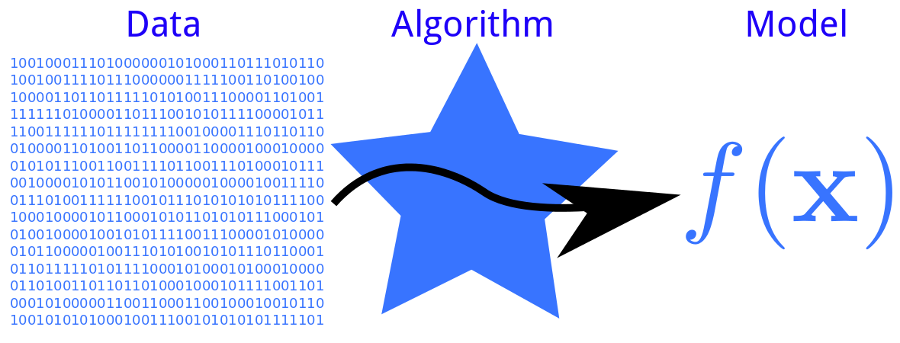
\includegraphics[keepaspectratio, width=0.75\textwidth]{graphics/steps}
	\end{figure}
\end{frame}

\begin{frame}
	\frametitle{Machine Learning Taxonomy\footnote[frame]{http://machinelearningmastery.com/a-tour-of-machine-learning-algorithms/}}
	\begin{description}
		\item[Supervised Learning] Input data has a known label or result such as spam\slash not-spam or a stock price at a time.
		\item[Unsupervised Learning] Input data is not labelled and does not have a known result.
		\item[Reinforcement Learning] Learns from the consequences of its actions, rather than from being explicitly taught. 
	\end{description}
\end{frame}

\begin{frame}
	\frametitle{Machine Learning Taxonomy}
	\begin{figure}
		\centering
		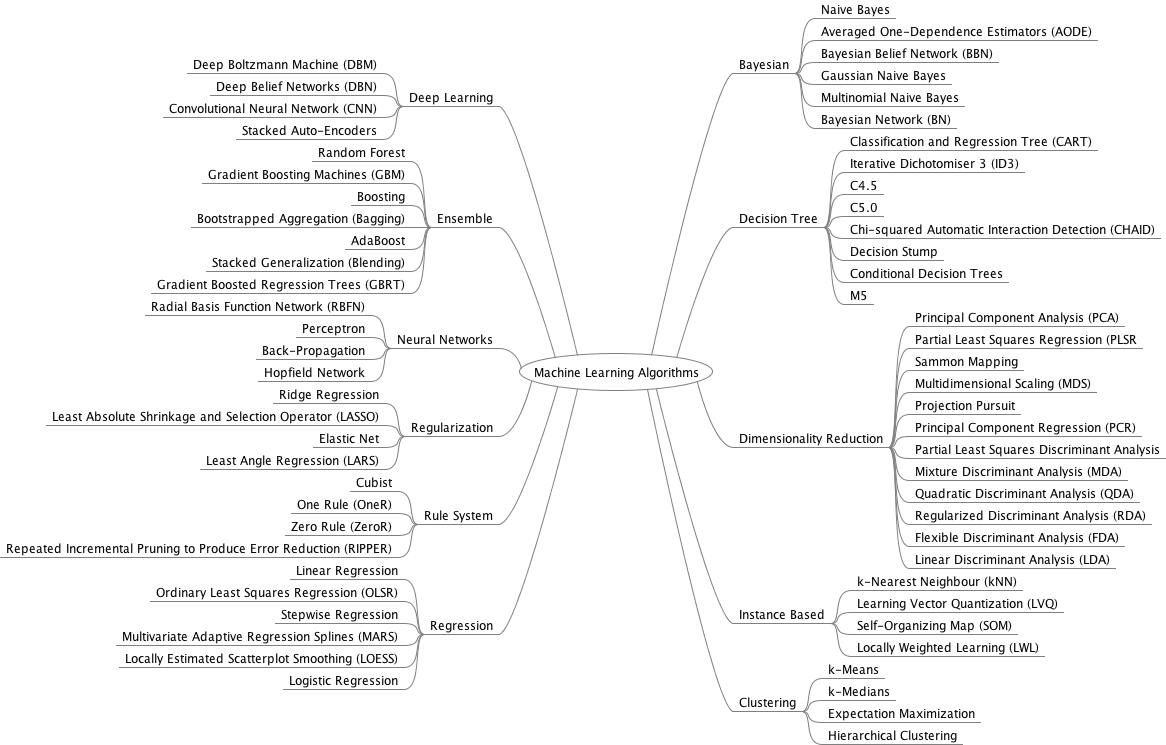
\includegraphics[keepaspectratio, width=0.95\textwidth]{graphics/MachineLearningAlgorithms}
	\end{figure}
\end{frame}

\section{Drawbacks}
\begin{frame}
\frametitle{Drawbacks}
\begin{itemize}
\item There is no silver bullet
\item There is no free lunch
\item Curse of dimensionality 
\end{itemize}
\end{frame}

\begin{frame}
	\frametitle{There is no silver bullet\footnote[frame]{http://www.pyimagesearch.com/2014/06/09/get-deep-learning-bandwagon-get-perspective/}}
	\begin{figure}
		\centering
		
\includegraphics[keepaspectratio, width=0.3\textwidth]{graphics/silverBullet}
	\end{figure}
\end{frame}

\begin{frame}
	\frametitle{There is no free lunch\footnote[frame]{http://www.no-free-lunch.org/}}
	\begin{quote}
	We have dubbed the associated results NFL theorems because they demonstrate that if an algorithm performs well on a certain class of problems then it necessarily pays for that with degraded performance on the set of all remaining problems.	
	\end{quote}
\end{frame}

\begin{frame}
	\frametitle{Curse of dimensionality\footnote[frame]{http://www.visiondummy.com/2014/04/curse-dimensionality-affect-classification/}}
\begin{quote}
	As the number of \emph{features} or \emph{dimensions} grows, the amount of data we need to generalize accurately grows \emph{exponentially}.
\end{quote}
\end{frame}

\section{Regression}
\begin{frame}
	\frametitle{Linear Regression}
	\begin{itemize}
		\item Model: $h_{\theta}(X) = \theta_0 + \theta_{1}X_{1} + ... + \theta_{n}X_{n}$
		\item Cost function: $J(\theta) = \frac{1}{2m}\sum_{i=1}^{m}(h_{\theta}(x^{(i)}-y^{(i)}))^{2}$
	\end{itemize}
	\begin{figure}
		\centering
		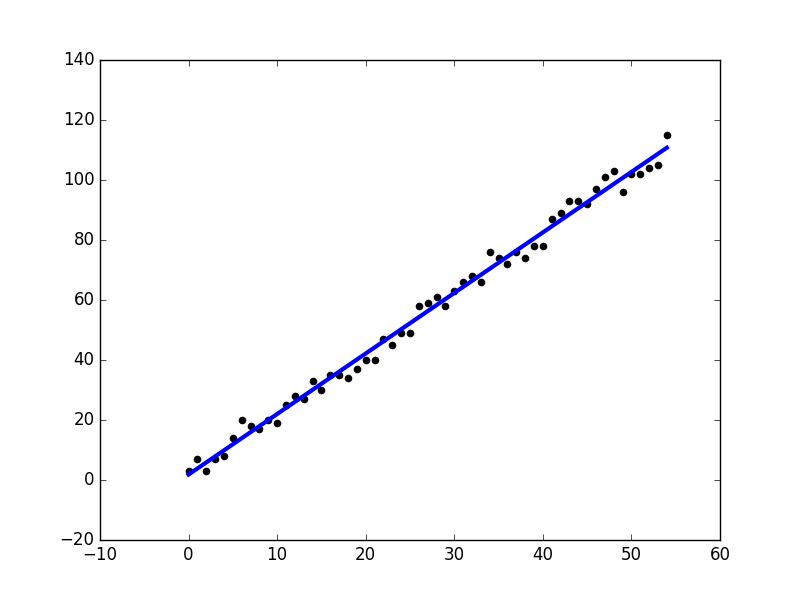
\includegraphics[keepaspectratio, width=0.65\textwidth]{graphics/linearRegression}
	\end{figure}
\end{frame}

\begin{frame}
	\frametitle{Gradient Descent\footnote[frame]{http://sebastianruder.com/optimizing-gradient-descent/}}
	\begin{itemize}
		\item Gradient descent is a way to minimize an objective function $J(\theta)$ parameterized by a model's parameters $\theta$ by updating the parameters in the opposite direction of the gradient. 
		\item Minimize: $\theta_{j} = \theta_{j} - \alpha \frac{\delta}{\delta \theta_{j}} J(\theta)$
	\end{itemize}
	\begin{figure}
		\centering
		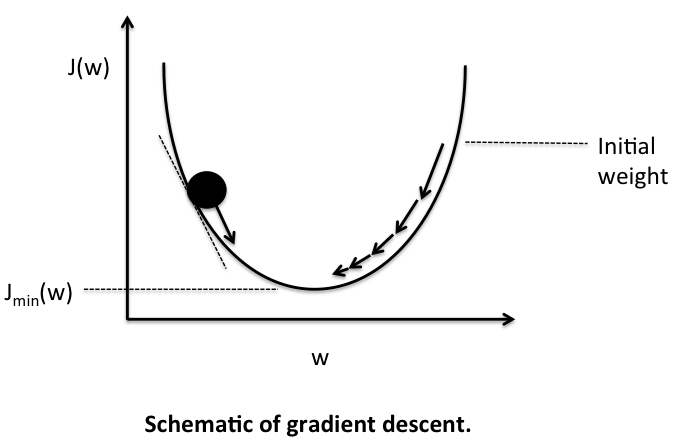
\includegraphics[keepaspectratio, width=0.55\textwidth]{graphics/gd}
	\end{figure}
\end{frame}

\section{Classification}
\begin{frame}
	\frametitle{Logistic Regression}
	\begin{itemize}
		\item Regression model where the dependent variable is categorical.
		\begin{itemize}
			\item If $h_{\theta}(X) \geq 0.5$ predict 1
			\item If $h_{\theta}(X) < 0.5$ predict 0
		\end{itemize}
	\end{itemize}
	\begin{figure}
		\centering
		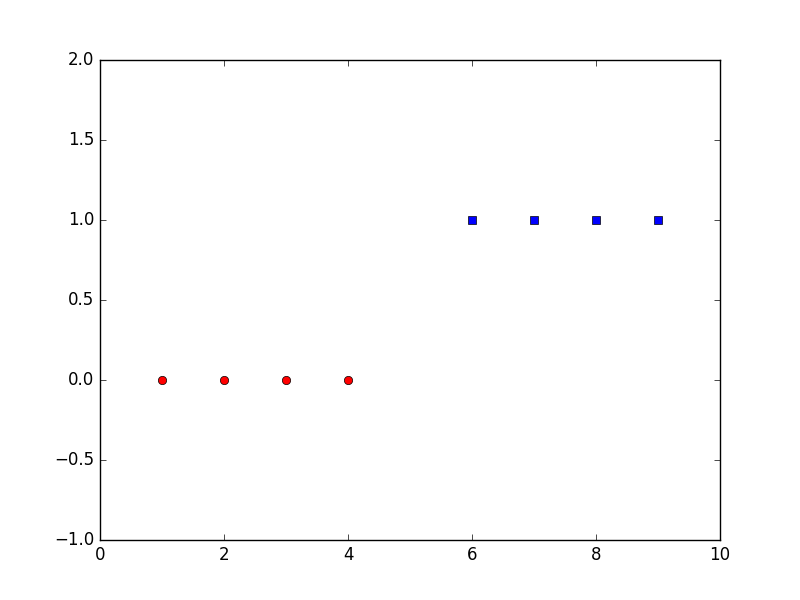
\includegraphics[keepaspectratio, width=0.55\textwidth]{graphics/logisticRegression00}
	\end{figure}
\end{frame}

\begin{frame}
	\frametitle{Logistic Regression}
	\begin{itemize}
		\item Want $0 \leq h_{\theta}(X) \leq 1$
		\item Sigmoid function: $g(Z) = \frac{1}{1+e^{-z}}$
		\item Model: $h_{\theta}(X) = g(\theta^{T}X)$
		\item $h_{\theta}(X)=$ estimated probability that $y=1$ on input $X$
	\end{itemize}
	\begin{figure}
		\centering
		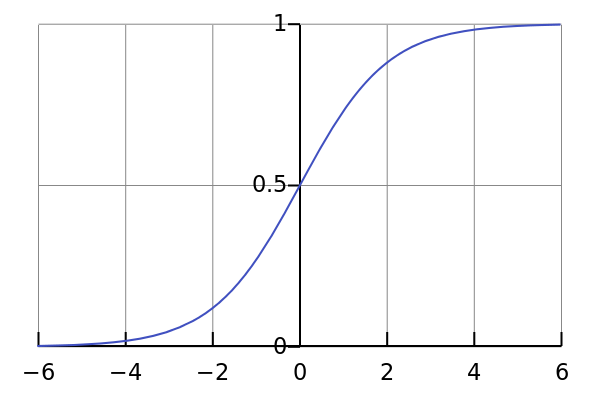
\includegraphics[keepaspectratio, width=0.55\textwidth]{graphics/sigmoid}
	\end{figure}
\end{frame}

\begin{frame}
	\frametitle{Logistic Regression}
	\begin{itemize}
		\item Cost function: $J(\theta) = \frac{1}{m}\sum_{i=1}^{m}Cost(h_{\theta}(x^{(i)}),y^{(i)}))$
		\item $Cost(h_{\theta}(x^{(i)}),y^{(i)}) = \left\{\begin{matrix}
		-log(h_{\theta}(x^{(i)}))\; if\; y=1\\ 
		-log(1-h_{\theta}(x^{(i)}))\; if\; y=0
		\end{matrix}\right.$
	\end{itemize}
	\begin{figure}
		\centering
		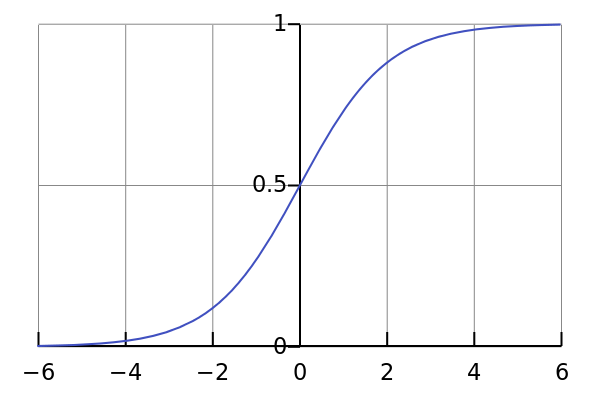
\includegraphics[keepaspectratio, width=0.55\textwidth]{graphics/sigmoid}
	\end{figure}
\end{frame}

\section{Clustering}
\begin{frame}
	\frametitle{K-means\footnote[frame]{http://www.onmyphd.com/?p=k-means.clustering}}
	\begin{itemize}
		\item Groups unlabeled data based on distance
		\item Minimizes: $min \sum_{i=1}^{k}\sum_{x \in C_{i}}  d(x, \mu)^{2}$
	\end{itemize}
	\begin{figure}
		\centering
		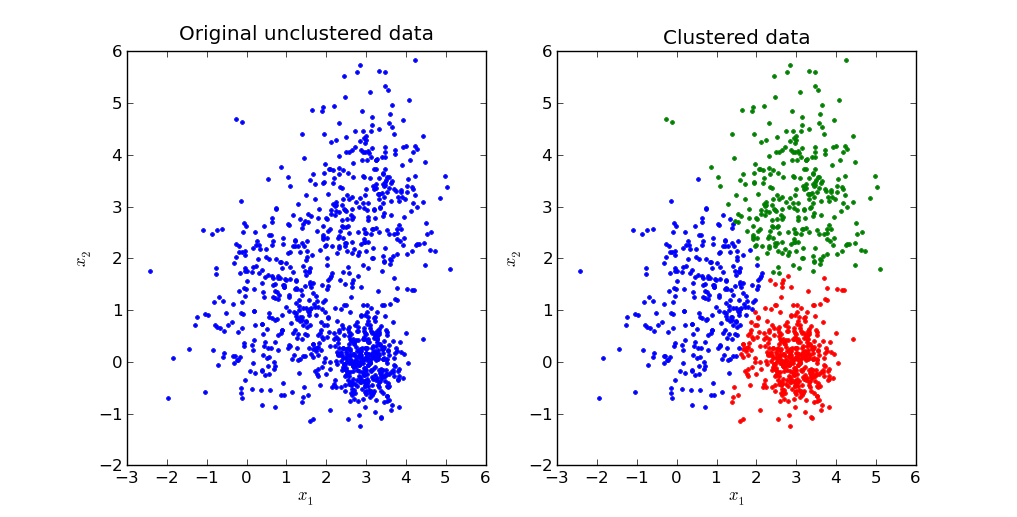
\includegraphics[keepaspectratio, width=0.65\textwidth]{graphics/kmeans_2d}
	\end{figure}
\end{frame}

\begin{frame}
	\frametitle{Choosing K in K-means}
	\begin{enumerate}
		\item Intuition about the problem
		\item Elbow method
		\item GAP statistic or equivalent
	\end{enumerate}
	\begin{figure}
		\centering
		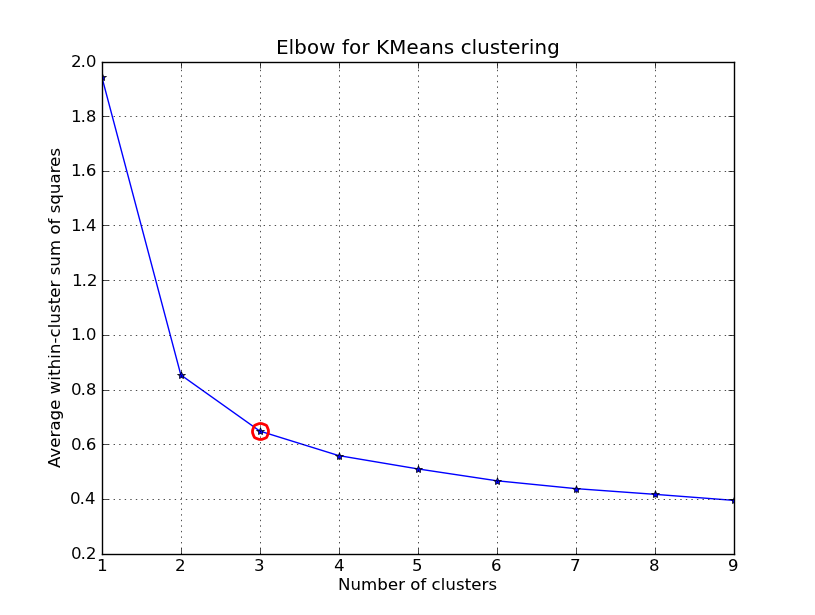
\includegraphics[keepaspectratio, width=0.45\textwidth]{graphics/elbow}
	\end{figure}
\end{frame}

\section{More about}
\begin{frame}
	\frametitle{More about}
	\begin{itemize}
		\item http://marketingland.com/how-machine-learning-works-150366
		\item http://www.learningmachines101.com/about-learning-machines-101/
		\item http://www.astroml.org/sklearn\_tutorial/general\_concepts.html
		\item https://www.coursera.org/learn/machine-learning/
	\end{itemize}
\end{frame}


\begin{frame}
\frametitle{End}
\begin{center}
	\begin{Large}
		END!!
	\end{Large}
\end{center}
\end{frame}
\end{document}